\chapter{Git Basics}
\label{cha:git_basics}
This chapter has every git command related to the basic VCS functionalities. After completing this chapter, the reader will be able to initialize and setup his own git repository, do basic versioning via committing changes and view the current status of the reader's current working directory.

\textit{Additional Information}: The git software uses a so-called \dq{}HEAD\dq{}-pointer to point at the latest commit of the git repository. So if a new commit is done, the HEAD will be updated to point at the new commit. Every commit points to its previous commit. An illustration of this is seen in (\ref{fig:branch_pointer}).

\newpage

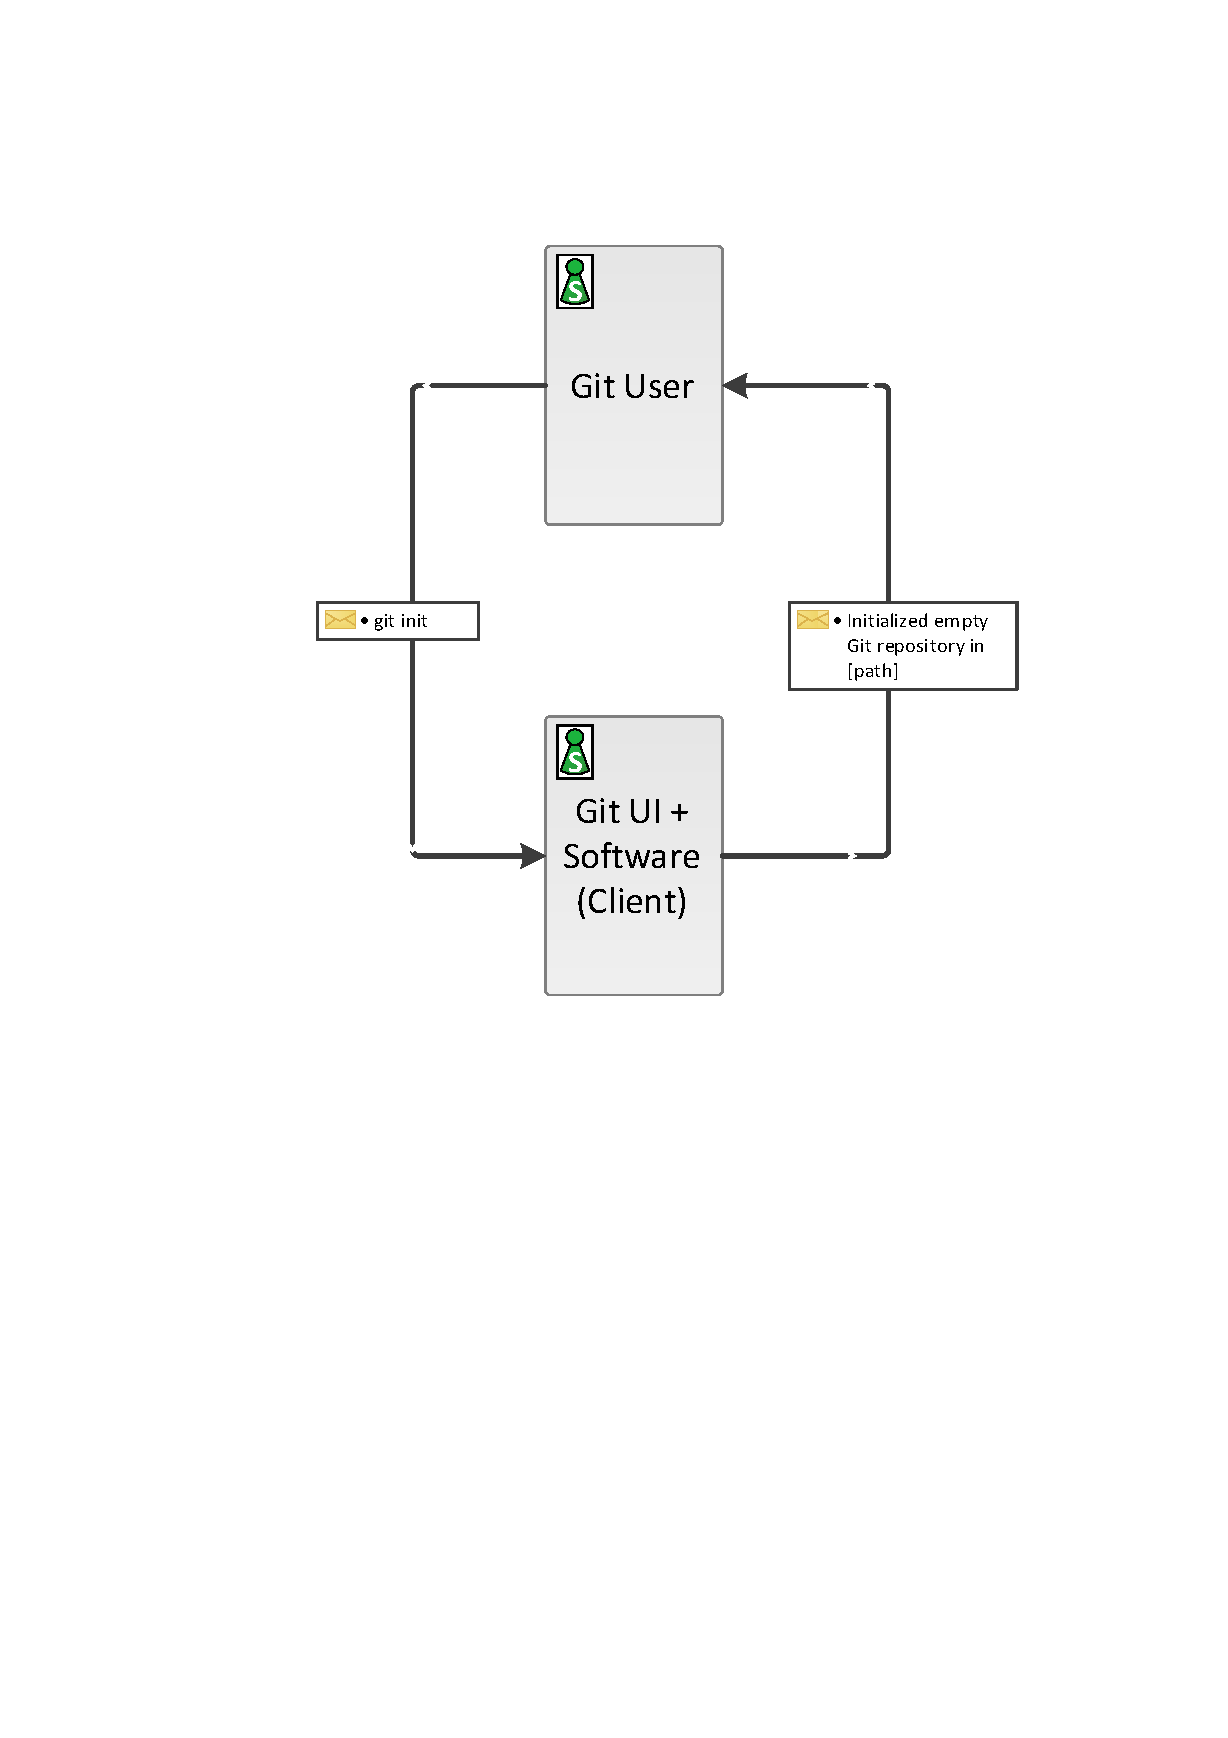
\includepdf[pages=1,pagecommand= {\section{git init} \label{sec:git_init}},scale=0.9]{git_commands/git_init.pdf}
\includepdf[pages=2-last,pagecommand={} ,scale=0.8]{git_commands/git_init.pdf}

\newpage

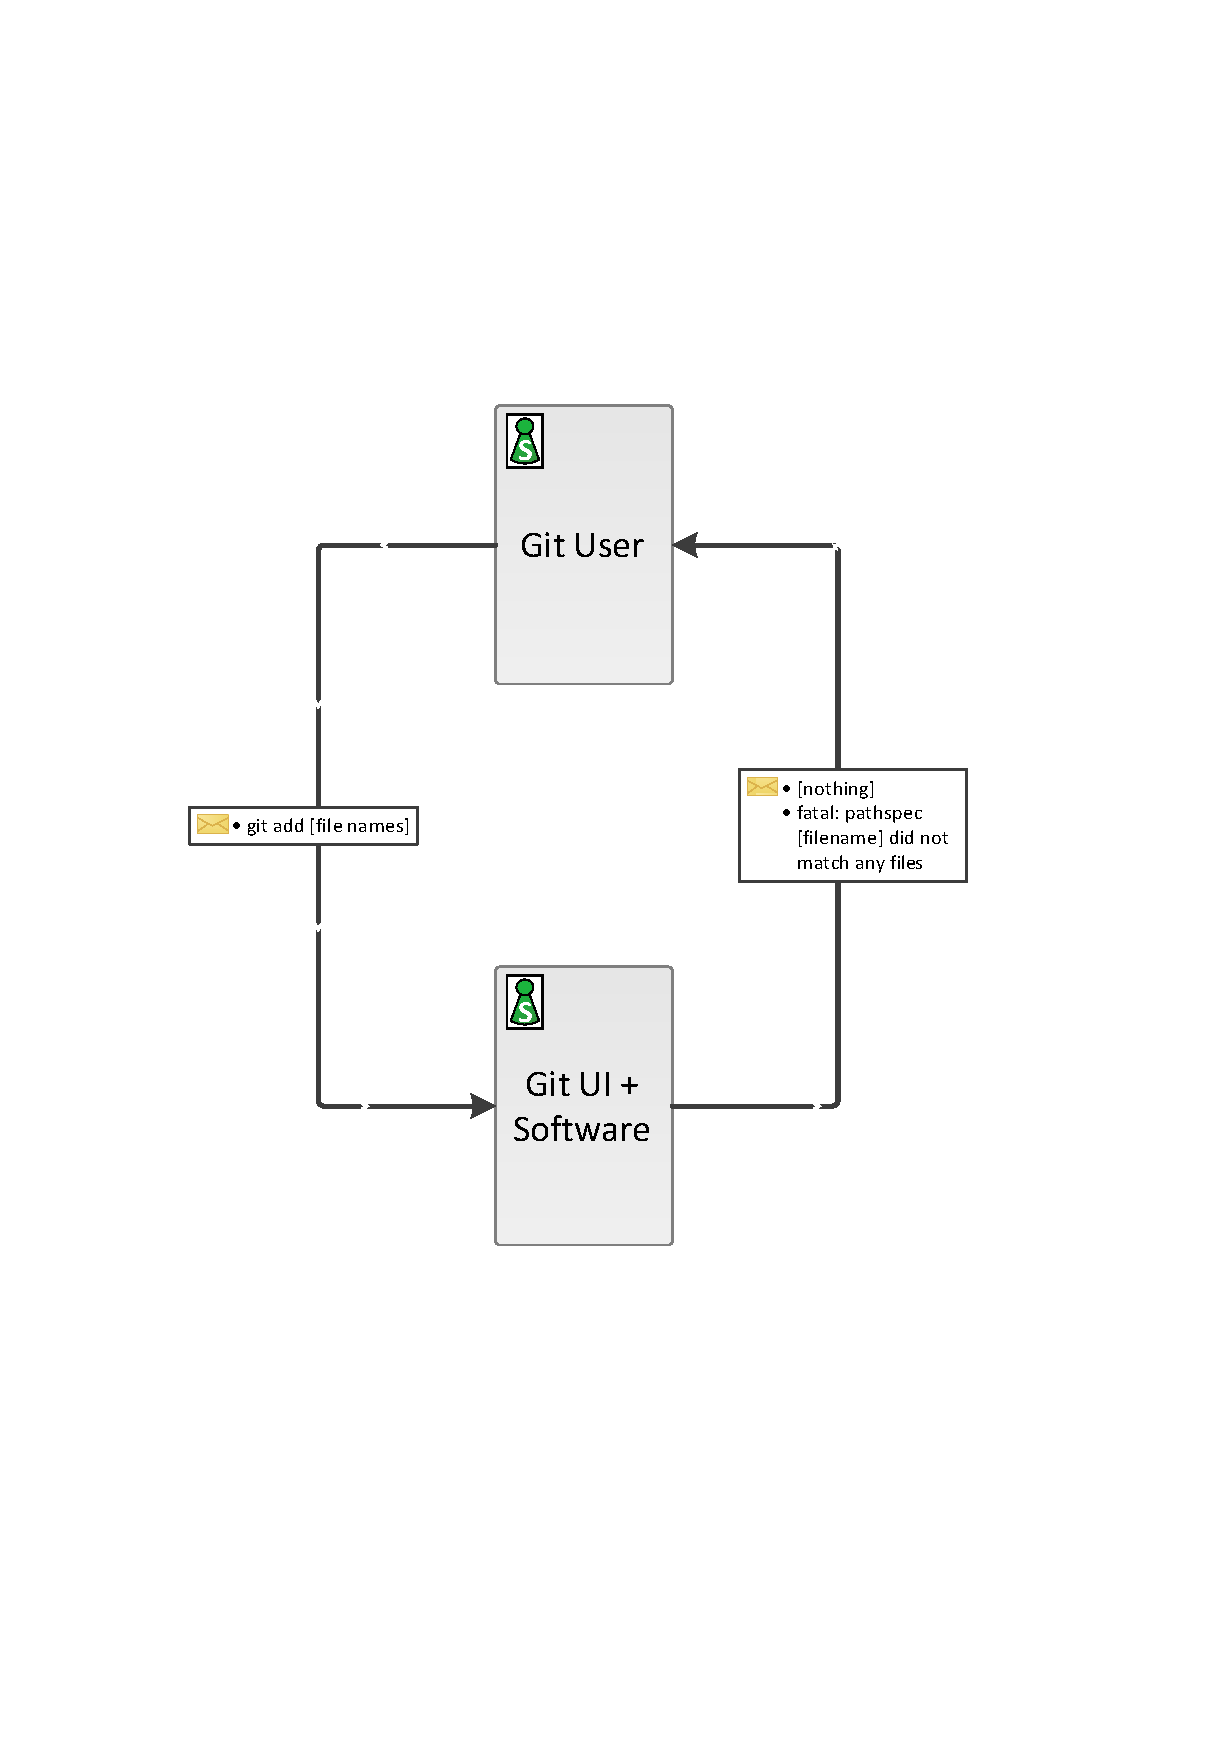
\includepdf[pages=1,pagecommand= {\section{git add} \label{sec:git_add}},scale=0.9]{git_commands/git_add.pdf}
\includepdf[pages=2-last,pagecommand={} ,scale=0.8]{git_commands/git_add.pdf}

\newpage

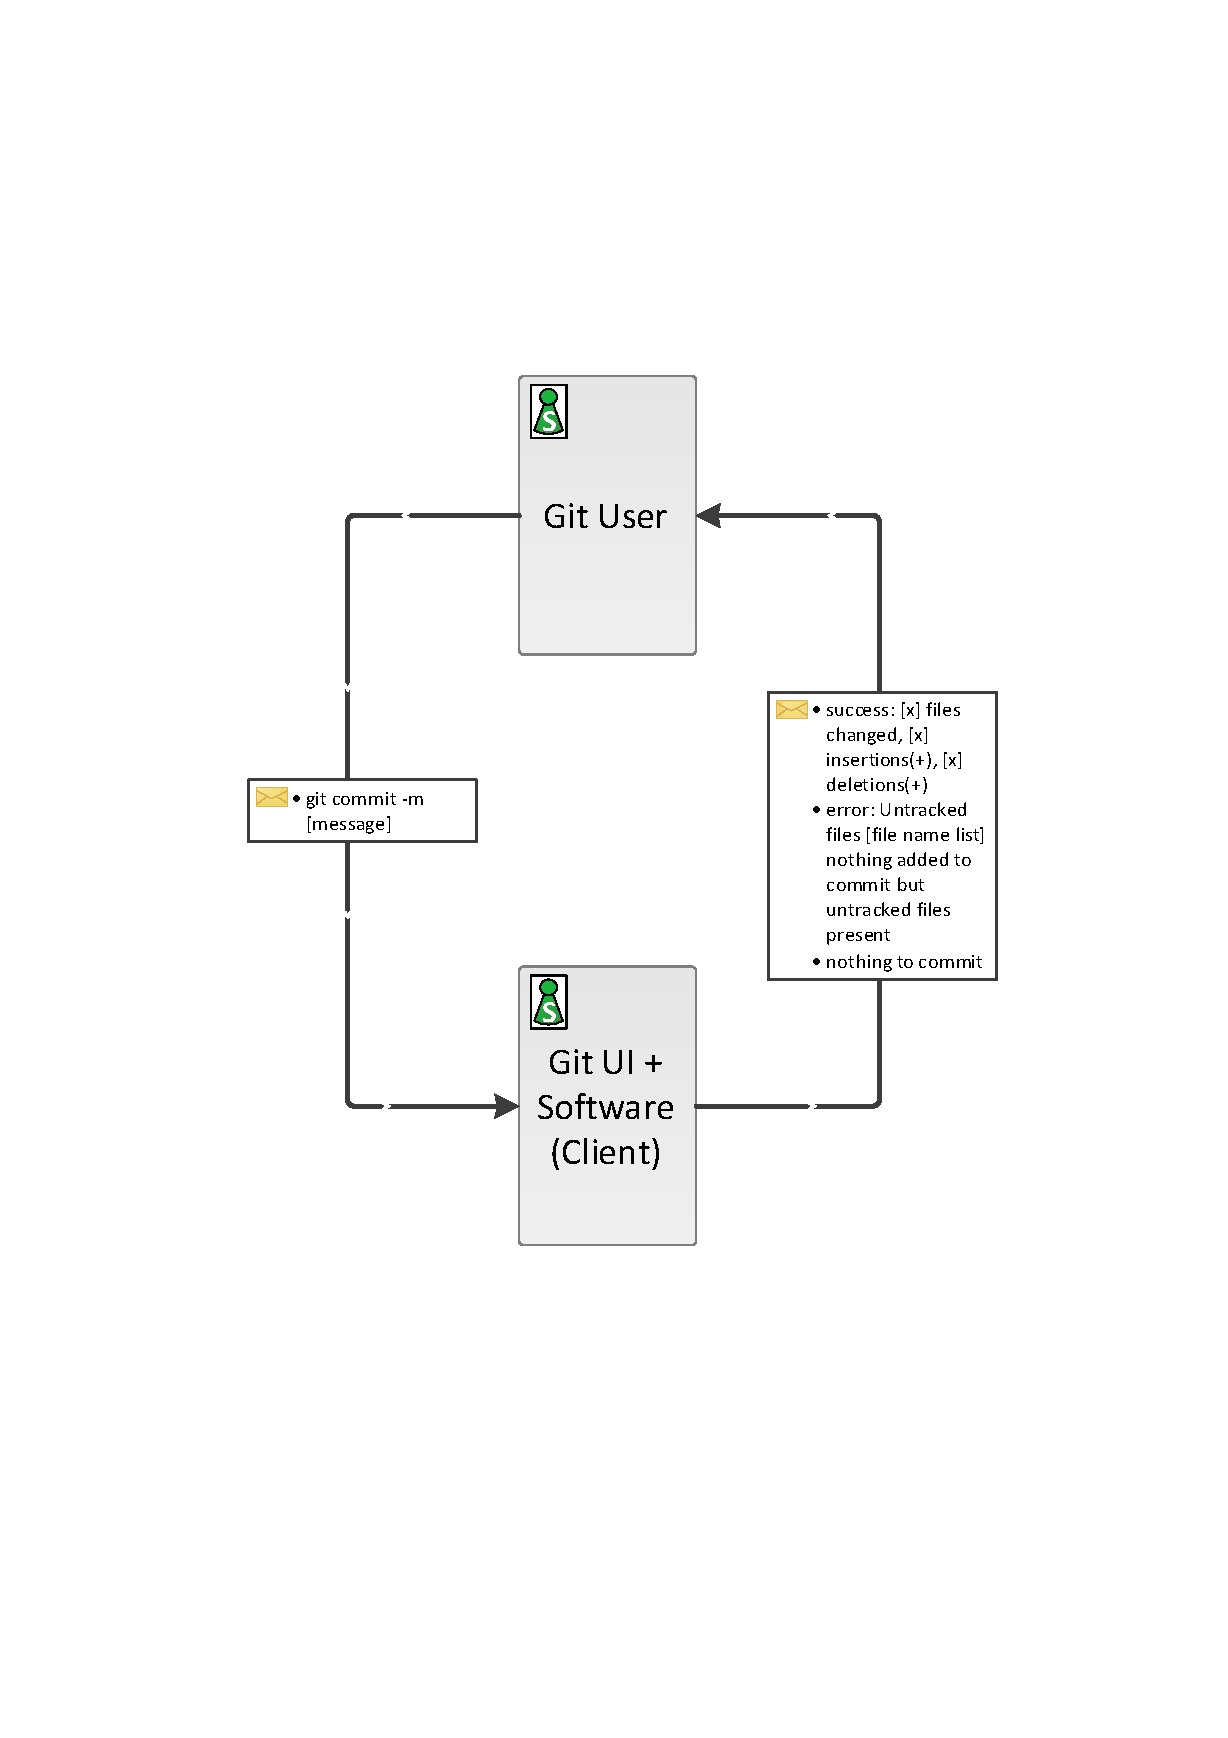
\includepdf[pages=1,pagecommand= {\section{git commit} \label{sec:git_commit}},scale=0.9]{git_commands/git_commit.pdf}
\includepdf[pages=2-last,pagecommand={} ,scale=0.8]{git_commands/git_commit.pdf}

\newpage

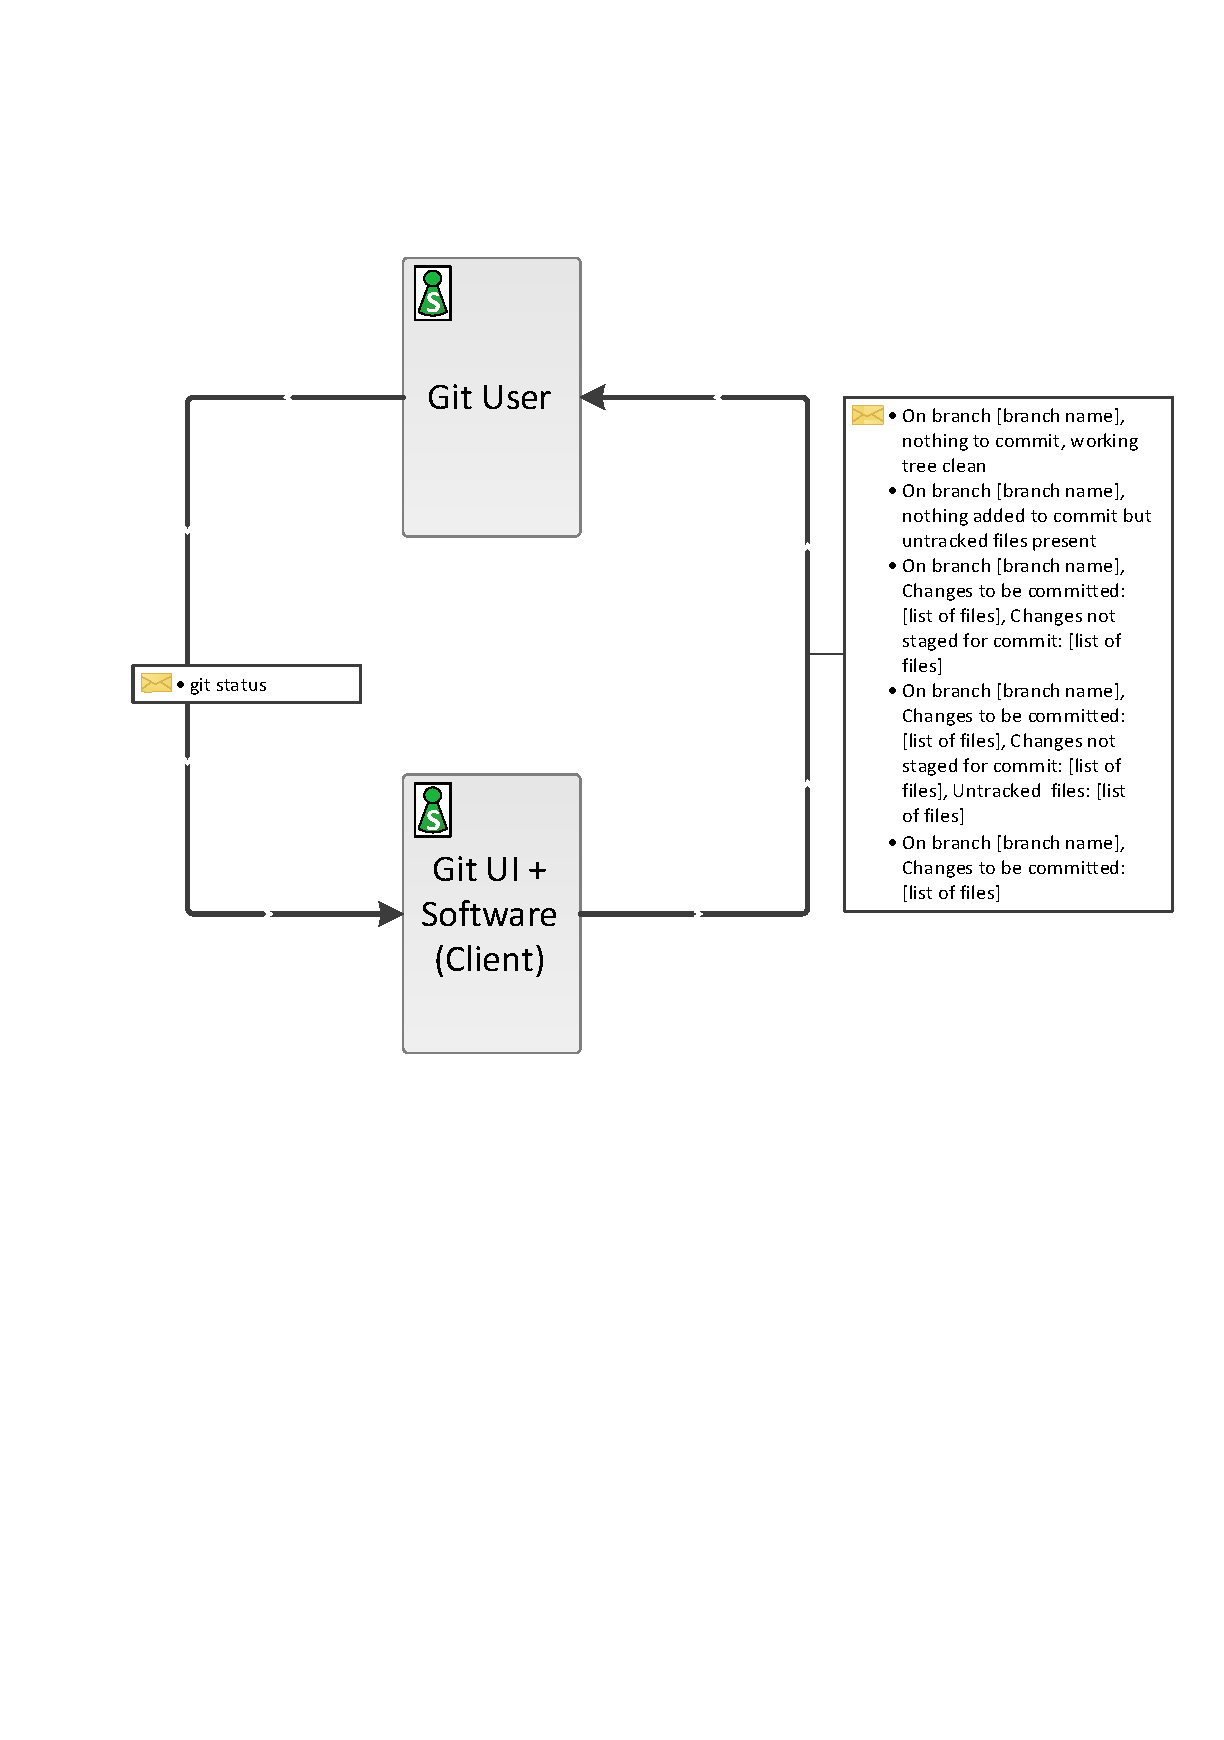
\includepdf[pages=1,pagecommand= {\section{git status} \label{sec:git_status} \subsection{git status local}},scale=0.9]{git_commands/git_status_local.pdf}
\includepdf[pages=2,pagecommand={} ,scale=0.78, angle = 270]{git_commands/git_status_local.pdf}
\includepdf[pages=3,pagecommand={} ,scale=0.75]{git_commands/git_status_local.pdf}
\newpage

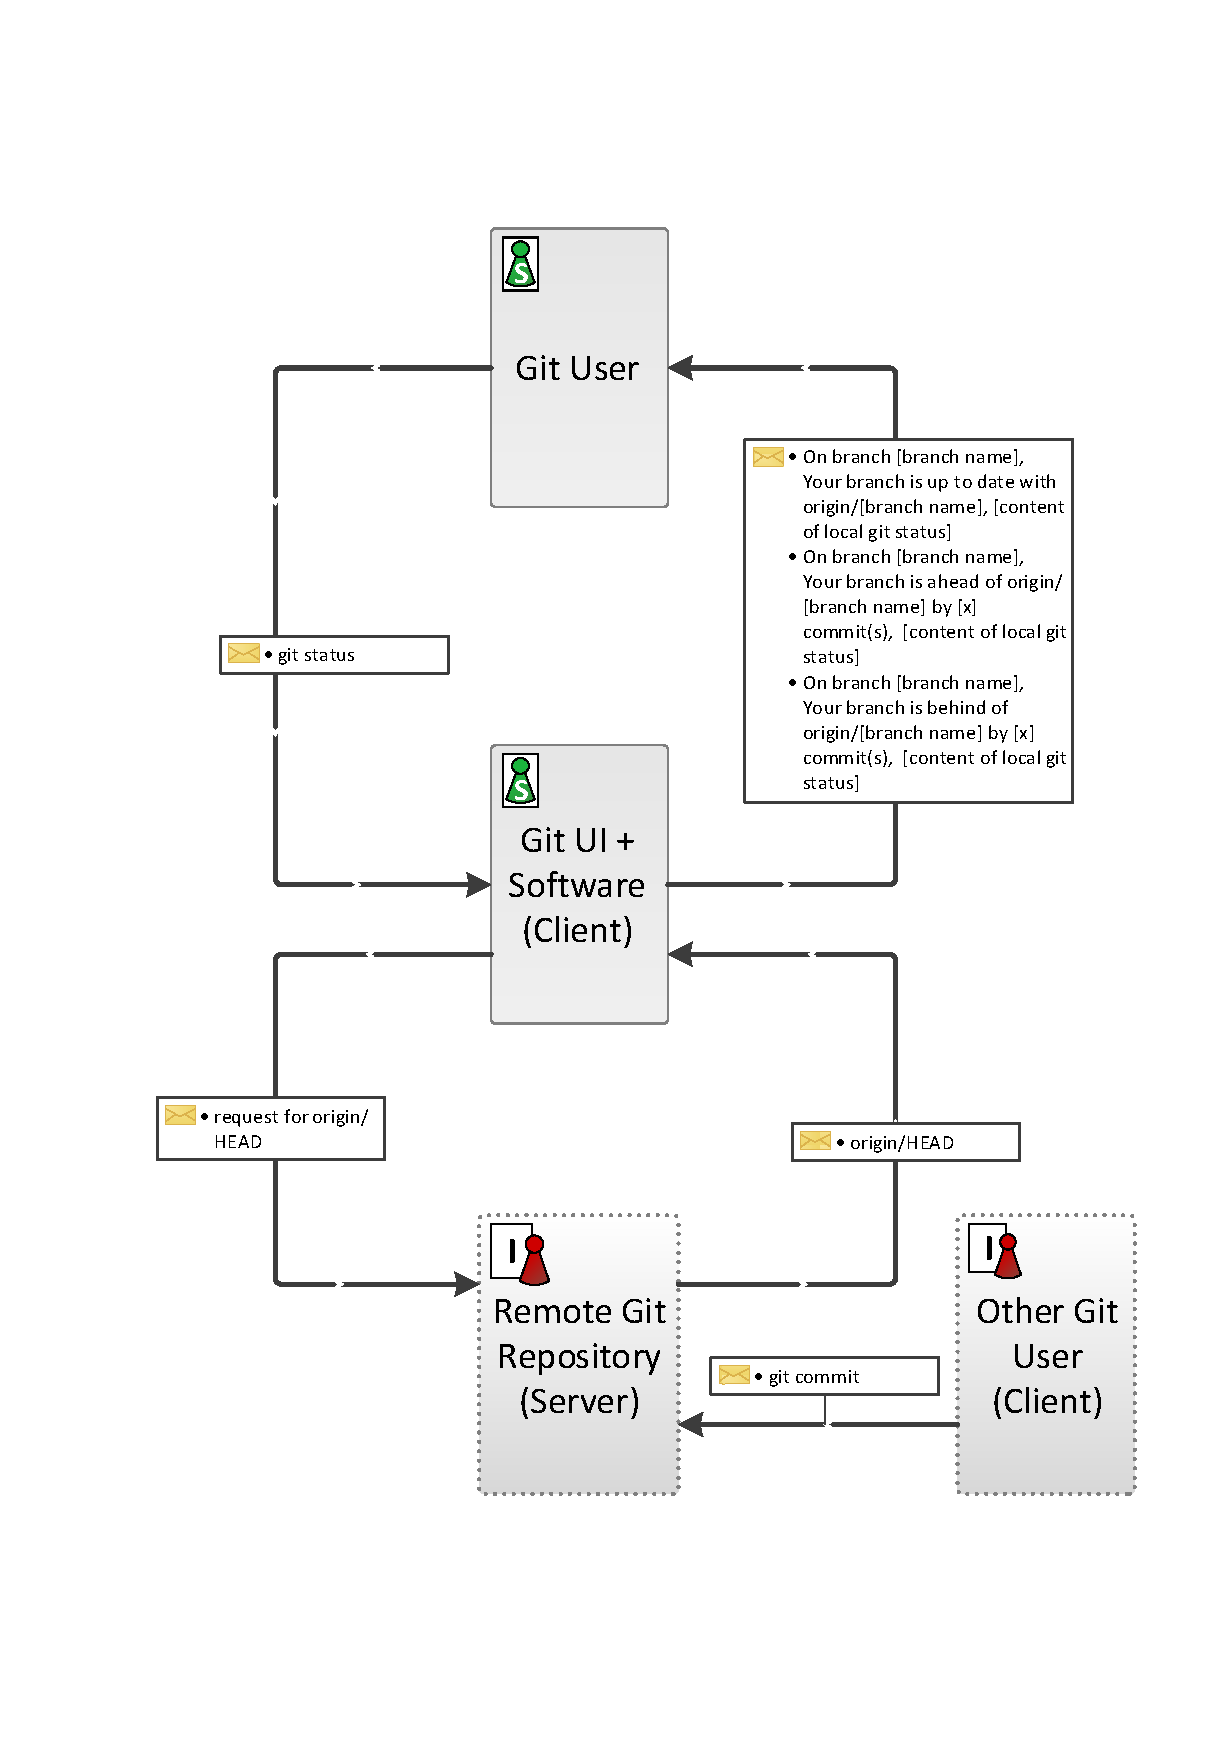
\includepdf[pages=1,pagecommand= {\subsection{git status remote}},scale=0.72]{git_commands/git_status_remote.pdf}
\includepdf[pages=2-last,pagecommand={} ,scale=0.75]{git_commands/git_status_remote.pdf}